\documentclass[12pt]{article}
\usepackage[letterpaper,left=4.9cm,right=1.9cm,top=3.1cm,bottom=2.3cm]{geometry} % Márgenes y demás
\usepackage[nswissgerman]{babel}
\usepackage{siunitx}
\usepackage[table]{xcolor}
\usepackage{dirtree}
\usepackage{pythonhighlight}
\usepackage[utf8]{inputenc}
\usepackage{pxfonts}
\usepackage{abstract}
\usepackage{parskip}
\usepackage{wasysym} % symbols
\usepackage{amssymb} % symbols
\usepackage{xcolor}
\usepackage[colorlinks=false]{hyperref}
%\usepackage{amsmath}
\usepackage{float}
\usepackage{graphicx}
\usepackage{fancyhdr}
\usepackage{titling}
\usepackage{hyperref}
\usepackage{svg}
\usepackage{caption}
\usepackage{titlesec}
\usepackage{apacite}
\usepackage[document]{ragged2e}
\usepackage[affil-sl]{authblk} 
\usepackage{mathptmx}  %Times new Roman 

\makeatletter


\renewcommand{\maketitle}{\bgroup\setlength{\parindent}{14pt}
\begin{flushleft}
  \textbf{\@title}
  \@author 
\end{flushleft}\egroup}

\makeatother

\pagestyle{fancy}
\fancyfoot[C]{}
\fancyfoot[R]{\thepage}
\renewcommand{\headrulewidth}{0pt}
\fancyhead{
  \fancyhead[R]{}
}




%%% Citaciones y año en negrilla
\renewcommand{\BAstyle}{\bfseries}
%%%%%%%%%%%%%%%%%%%%%%%%%%%%%%%%%%

%%%%%%% Número de volúmen en negrilla
\renewcommand{\APACjournalVolNumPages}[4]{%
  \Bem{#1}%             journal
  \ifx\@empty#2\@empty
  \else
    \unskip, \textbf{\Bem{#2}}%  volume
  \fi
  \ifx\@empty#3\@empty
  \else
    \unskip({#3})%      issue number
  \fi
  \ifx\@empty#4\@empty
  \else
    \unskip, {#4}%      pages
  \fi
}
%%%%%%%%%%%%%%%%%%%


%%%%% Nombres de los autores en negrilla
\renewcommand{\APACrefauthstyle}{\bfseries}
%%%%%%%%%%%%%%%%%%%%%%%%%%%%%%%%%%%%%%%%



%% Comandos modificados al estilo
\renewcommand\Affilfont{\fontsize{8}{8}}

%%Tamaño fuente filiación 

\definecolor{bluesrev}{HTML}{136f8b}

\renewcommand{\absnamepos}{flushleft}
\renewcommand{\abstractnamefont}{\fontsize{13}{13}\bfseries}
\renewcommand{\abstracttextfont}{\fontsize{9}{1}\justifying}

\titleformat*{\section}{\fontsize{13}{1}\bfseries\color{bluesrev}}

\titleformat{\subsection} 
	{\normalfont\itshape }{\makebox[30pt][l]{\thesubsection}}{0pt}{}

\captionsetup{justification   = raggedright,
              singlelinecheck = false}

\captionsetup{labelfont=bf}
\captionsetup{labelsep=period}


\renewcommand{\figurename}{Figura}


%%% ORCID  %%%

\usepackage{scalerel}
\usepackage{tikz}

\definecolor{orcidlogocol}{HTML}{A6CE39}

%%%%%%%%%%%%%%%%%%%


  

\setlength{\topskip}{0.5cm}
\setlength{\parindent}{0mm}

%\title{\fontsize{14}{14}\textbf{Sleep Cube - Diary} \\[0.2cm]

\title{\textcolor{gray}{\textbf{sleepCube - Programme/Aufbau}\\[0.2cm]}}



\author[1]{\fontsize{9}{9} \textbf{Ugur Turhal}}
%\author[2]{\textbf{Silvan Lenzlinger}}
%\author[1]{\textbf{Berkan Kurt}}

\affil[1]{\fontsize{8}{8}\href{mailto:ugur.turhal@me.com}{ugur.turhal@me.com}}
\date{\today}                     
\setcounter{Maxaffil}{0}

\usepackage{listings,newtxtt}

\lstset{basicstyle=\ttfamily, keywordstyle=\bfseries}    

\definecolor{mygreen}{rgb}{0,0.6,0}
\definecolor{mygray}{rgb}{0.47,0.47,0.33}
\definecolor{myorange}{rgb}{0.8,0.4,0}
\definecolor{mywhite}{rgb}{0.98,0.98,0.98}
\definecolor{myblue}{rgb}{0.01,0.61,0.98}

\lstnewenvironment{code}{\lstset{ %
  backgroundcolor=\color{mywhite},   
  basicstyle=\footnotesize,       
  breakatwhitespace=false,         
  breaklines=true,                 
  captionpos=b,                   
  commentstyle=\color{mygray},    
  deletekeywords={...},           
  escapeinside={\%*}{*)},          
  extendedchars=true,              
  frame=shadowbox,                    
  keepspaces=true,                 
  keywordstyle=\color{myorange},       
  language=C++,                
  morekeywords={*,...},            
  numbers=left,                    
  numbersep=5pt,                   
  numberstyle=\tiny\color{mygray}, 
  rulecolor=\color{black},         
  rulesepcolor=\color{myblue},
  showspaces=false,                
  showstringspaces=false,          
  showtabs=false,                  
  stepnumber=2,                    
  stringstyle=\color{myorange},    
  tabsize=2,                       
  title=\lstname                   
}}{}

\DeclareSIUnit \volt{V} %apparent power 
\begin{document}
\maketitle
\tableofcontents
\addtocontents{toc}{\protect\thispagestyle{empty}}
\newpage
\setcounter{page}{1}
\section{DHT22}
\justifying
Der Sensor ist ein DHT22, welcher wie folgt aus sieht. Mit diesem wird die Umgebungstemperatur gemessen. Der DHT22 hat 4 Pins siehe Bild \ref{Fig:description}. Dessen Erläuterung ist in der Tabelle\ref{Tabular:pins}.
\begin{figure}[H]
\begin{center}
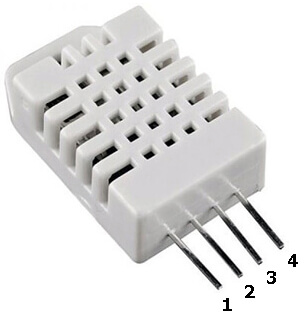
\includegraphics[width = 0.25\textwidth]{pics/DHT22.jpg}
\caption{DHT22 - Pins}
\label{Fig:description}
\end{center}
\end{figure}
\subsection{Pins und deren Bedeutung}
\begin{table}[H]
\centering
\rowcolors{2}{purple!30}{pink!60}
\begin{tabular}{l|l}
\textbf{Pin} & \textbf{Funktion}\\ \hline \hline
1 & Betriebsspannung (3,3V - 5,5V) \\ \hline
2 & Serial Data Line\\\hline
3 & Nicht belegt\\ \hline
4 & Ground
\end{tabular}
\caption{Pins - Bedeutung}
\label{Tabular:pins}
\end{table}
\subsection{Verkabelung}
\begin{figure}[H]
\begin{center}
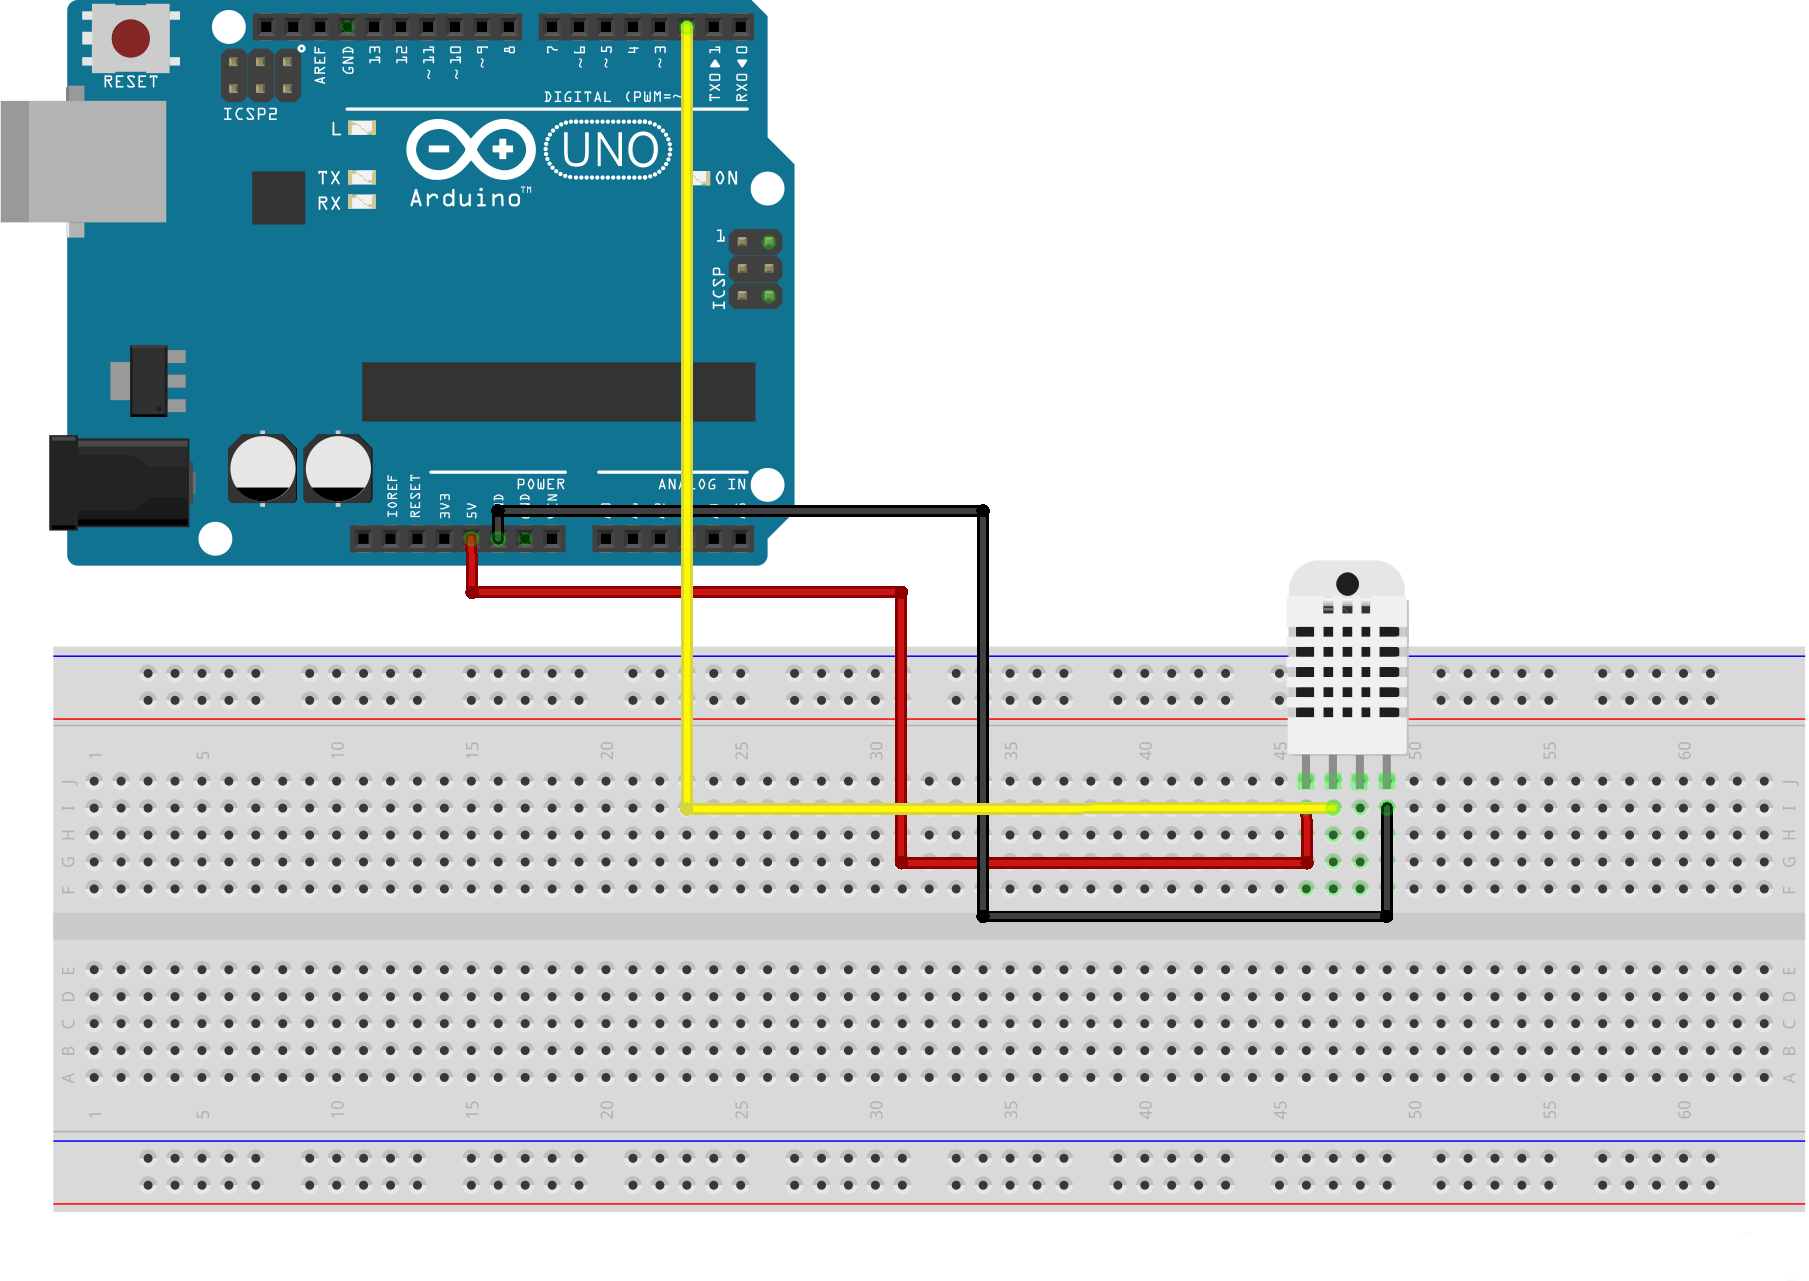
\includegraphics[width=0.5\textwidth]{pics/wireddht.png}
\caption{DHT mit Arduino UNO verbunden}
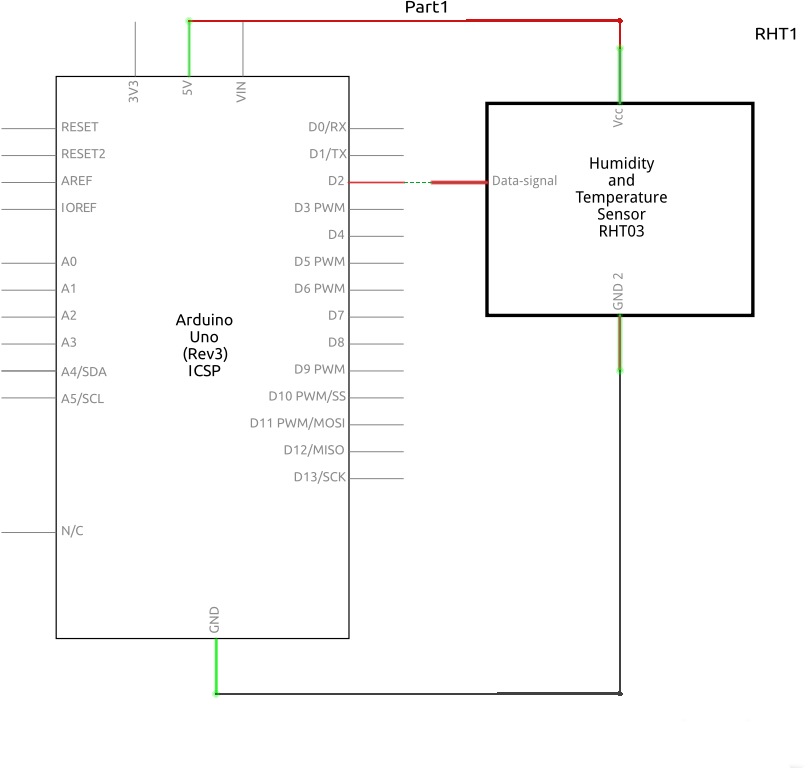
\includegraphics[width=0.5\textwidth]{pics/schematic.png}
\caption{Schaltplan DHT22 und Arduino UNO}
\end{center}
\end{figure}
\section{DHT22 - Arduino}
\justifying
Installiere die DHT sensor library in die Arduino IDE:
\begin{figure}[H]
\DTsetlength{0.2em}{2.5em}{0.2em}{0.4pt}{2.6pt}
\dirtree{%
.1 /.
.2 Tools.
.3 Manage Libraries$\dots$ .
.4 Mangae Library.
.5 \textit{Filter your Search}.
.6 DHT22.
.6 \textbf{DHT22 sensor library}\\ by Adafruit Version 1.4.3.
}
\end{figure}
%%%%%%%%%%%%%%%%%%%%%%%%%%%%%%%%%%%%%%%%%%%%%%%%%%%%%%%%%%%%%%%%%%%%%%%%%%%%%%%%%%%%%%%%%%%%%%%%%%%%%%%%%%%%%%%%%%%%%%%%%%%%%%%%%%%%%%%%%%%%%%%%%%%%%%%%%%%%%%%%%%%%
DHT22 ist bereit zum Einsatz.

\subsection{Arduino Code}
\begin{code}
#include "DHT.h"

#define DHTPIN 2 //Pin Nummer wo der Sensor angeschlossen ist
#define DHTTYPE DHT22 //Definition was fuer ein Sensor ausgelesen wird.

DHT dht(DHTPIN, DHTTYPE);

void setup() {
  // put your setup code here, to run once:
  Serial.begin(9600);
  //Serial.println("DHT22 Testprogramm");
  dht.begin();

}

void loop() {
  delay(2000);                     
                                    
  float h = dht.readHumidity();    
  float t = dht.readTemperature();
  
  if (isnan(h) || isnan(t)) {       
    Serial.println("Fehler beim auslesen des Sensors!");
    return;
  }

                   
  Serial.print(h);                 
  Serial.print(" ");                          
  Serial.println(t);
}
\end{code}
\newpage
\subsection{Python and Arduino}
Zwei Python Programme wurden geschrieben um Daten aufzunehmen und zu visualisieren.
\begin{python}[language=Python]
# @author Ugur Turhal
# This python file reads the serial port of the Arduino and gives a live plot
import serial
import time
import csv
import matplotlib
import matplotlib.pyplot as plt
import numpy as np

matplotlib.use("tkAgg")
ser = serial.Serial('/dev/ttyACM0')
ser.flushInput()

plot_window = 360
y_var = np.array(np.zeros([plot_window]))
plt.ion()
fig, ax = plt.subplots()
ax.grid(linestyle="--")
ax.set_ylabel("Celsius")
ax.set_xlabel("x")
ax.set(xlabel='x', ylabel='Celsius',
       title='Increase & Decrease of \n Temperature')
line, = ax.plot(y_var)

while True:
    try:
        ser_bytes = ser.readline()
        try:
            decoded_bytes = ser_bytes[0:len(ser_bytes) - 2].decode("utf-8")
            print(decoded_bytes)
        except:
            continue
        with open("test_data.csv", "a") as f:
            writer = csv.writer(f, delimiter=",")
            writer.writerow([time.time(), decoded_bytes])
        y_var = np.append(y_var, decoded_bytes)
        y_var = y_var[1:plot_window + 1]
        line.set_ydata(y_var)
        ax.relim()
        ax.autoscale_view()
        fig.canvas.draw()
        fig.canvas.flush_events()
        fig.savefig('full_figure.png')
    except:
        print("Stopped")
        break
\end{python}
\newpage
\begin{python}
# @author Ugur Turhal
# This python skript reads a CSV file, which
# is filtered and Plots in a log Plot the temperature

import numpy as np
import pandas as pd
import matplotlib.pyplot as plt

plt.style.use('seaborn')


def main():
    df = pd.read_csv("groupeddata.csv", usecols=['Measurement', 'Temperature']).drop_duplicates(keep='first').reset_index()
    measurement = df['Measurement']
    temperature = df['Temperature']
    df.to_csv("cleanData.csv");
    colors = [1, 2, 3, 4, 5, 6, 7, 8, 9, 10, 11, 12, 13, 14, 15, 16, 17, 18, 19, 20, 21, 22, 23, 24, 25, 26, 27, 28, 29, 30, 31, 32, 33, 34, 35, 36, 37, 38, 39, 40, 41, 42, 43, 44, 45, 46, 47, 48, 49, 50, 51, 52, 53, 54, 55, 56, 57, 58, 59, 60, 61, 62, 63, 64, 65, 66, 67, 68, 69, 70, 71, 72, 73, 74, 75, 76, 77, 78, 79, 80, 81, 82, 83, 84, 85, 86, 87, 88, 89, 90]

    plt.scatter(x=measurement, y=temperature, s=25, c=colors, alpha=0.6, edgecolor='black', linewidth=1,
                    cmap='Blues_r')

    cbar = plt.colorbar()
    cbar.set_label('Mesurements with Temperature')
    plt.xscale('log')
    plt.yscale('log')
    plt.title('Scatter of Temperature')
    plt.xlabel('Measurement')
    plt.ylabel('Temperature')

    plt.savefig("data.png")
    plt.show()


if __name__ == "__main__":
    print(main())

\end{python}
\subsection{Plots}
Für die Erklärung siehe: \url{https://github.com/ugurtu/CatcProject/blob/main/Bericht/bericht.pdf}
\begin{figure}[H]
\begin{center}
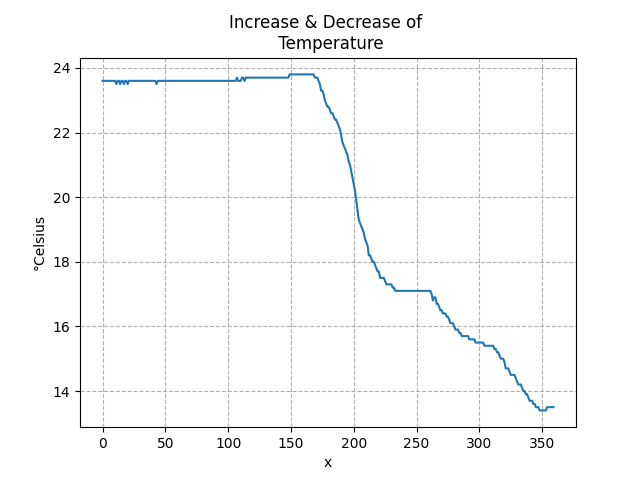
\includegraphics[width=0.7\textwidth]{pics/plot.png}
\caption{Temperaturausgaben über eine bestimme Zeit}
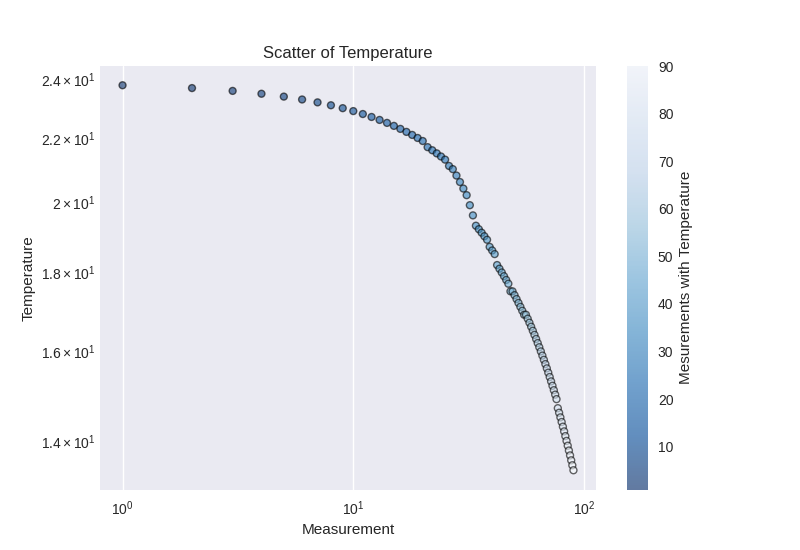
\includegraphics[width=0.7\textwidth]{pics/scatter.png}
\caption{Einzelne Messpunkte des DHT22}
\end{center}
\end{figure}
\newpage
\section{Simples Modell}
Arduino:
\begin{code}
#include "DHT.h"

#define DHTPIN 2 //Pin Nummer wo der Sensor angeschlossen ist
#define DHTTYPE DHT22 //Definition was fuer ein Sensor ausgelesen wird.
#define pinRed 4 // LEDPin4
#define pinGreen 5 //LEDPin5

DHT dht(DHTPIN, DHTTYPE);

void setup() {
  // put your setup code here, to run once:
  Serial.begin(9600);
  //Serial.println("DHT22 Testprogramm");
  pinMode(pinRed, OUTPUT);
  pinMode(pinGreen, OUTPUT);

  dht.begin();

}

void loop() {
  delay(2000);

  float h = dht.readHumidity();
  float t = dht.readTemperature();

  if (isnan(h) || isnan(t)) {
    Serial.println("Fehler beim auslesen des Sensors!");
    return;
  }

  if (t >= 15.00 && t <= 18.00) {
    digitalWrite(pinRed, LOW);
    digitalWrite(pinGreen, HIGH);
  }
  else  {
    digitalWrite(pinGreen,LOW);
    digitalWrite(pinRed, HIGH);    
  }   
   Serial.print(digitalRead(pinRed));
   Serial.print(" ");
   Serial.print(digitalRead(pinGreen));
   Serial.print(" ");
   Serial.println(t);
}
\end{code}
\begin{figure}[H]
\begin{center}
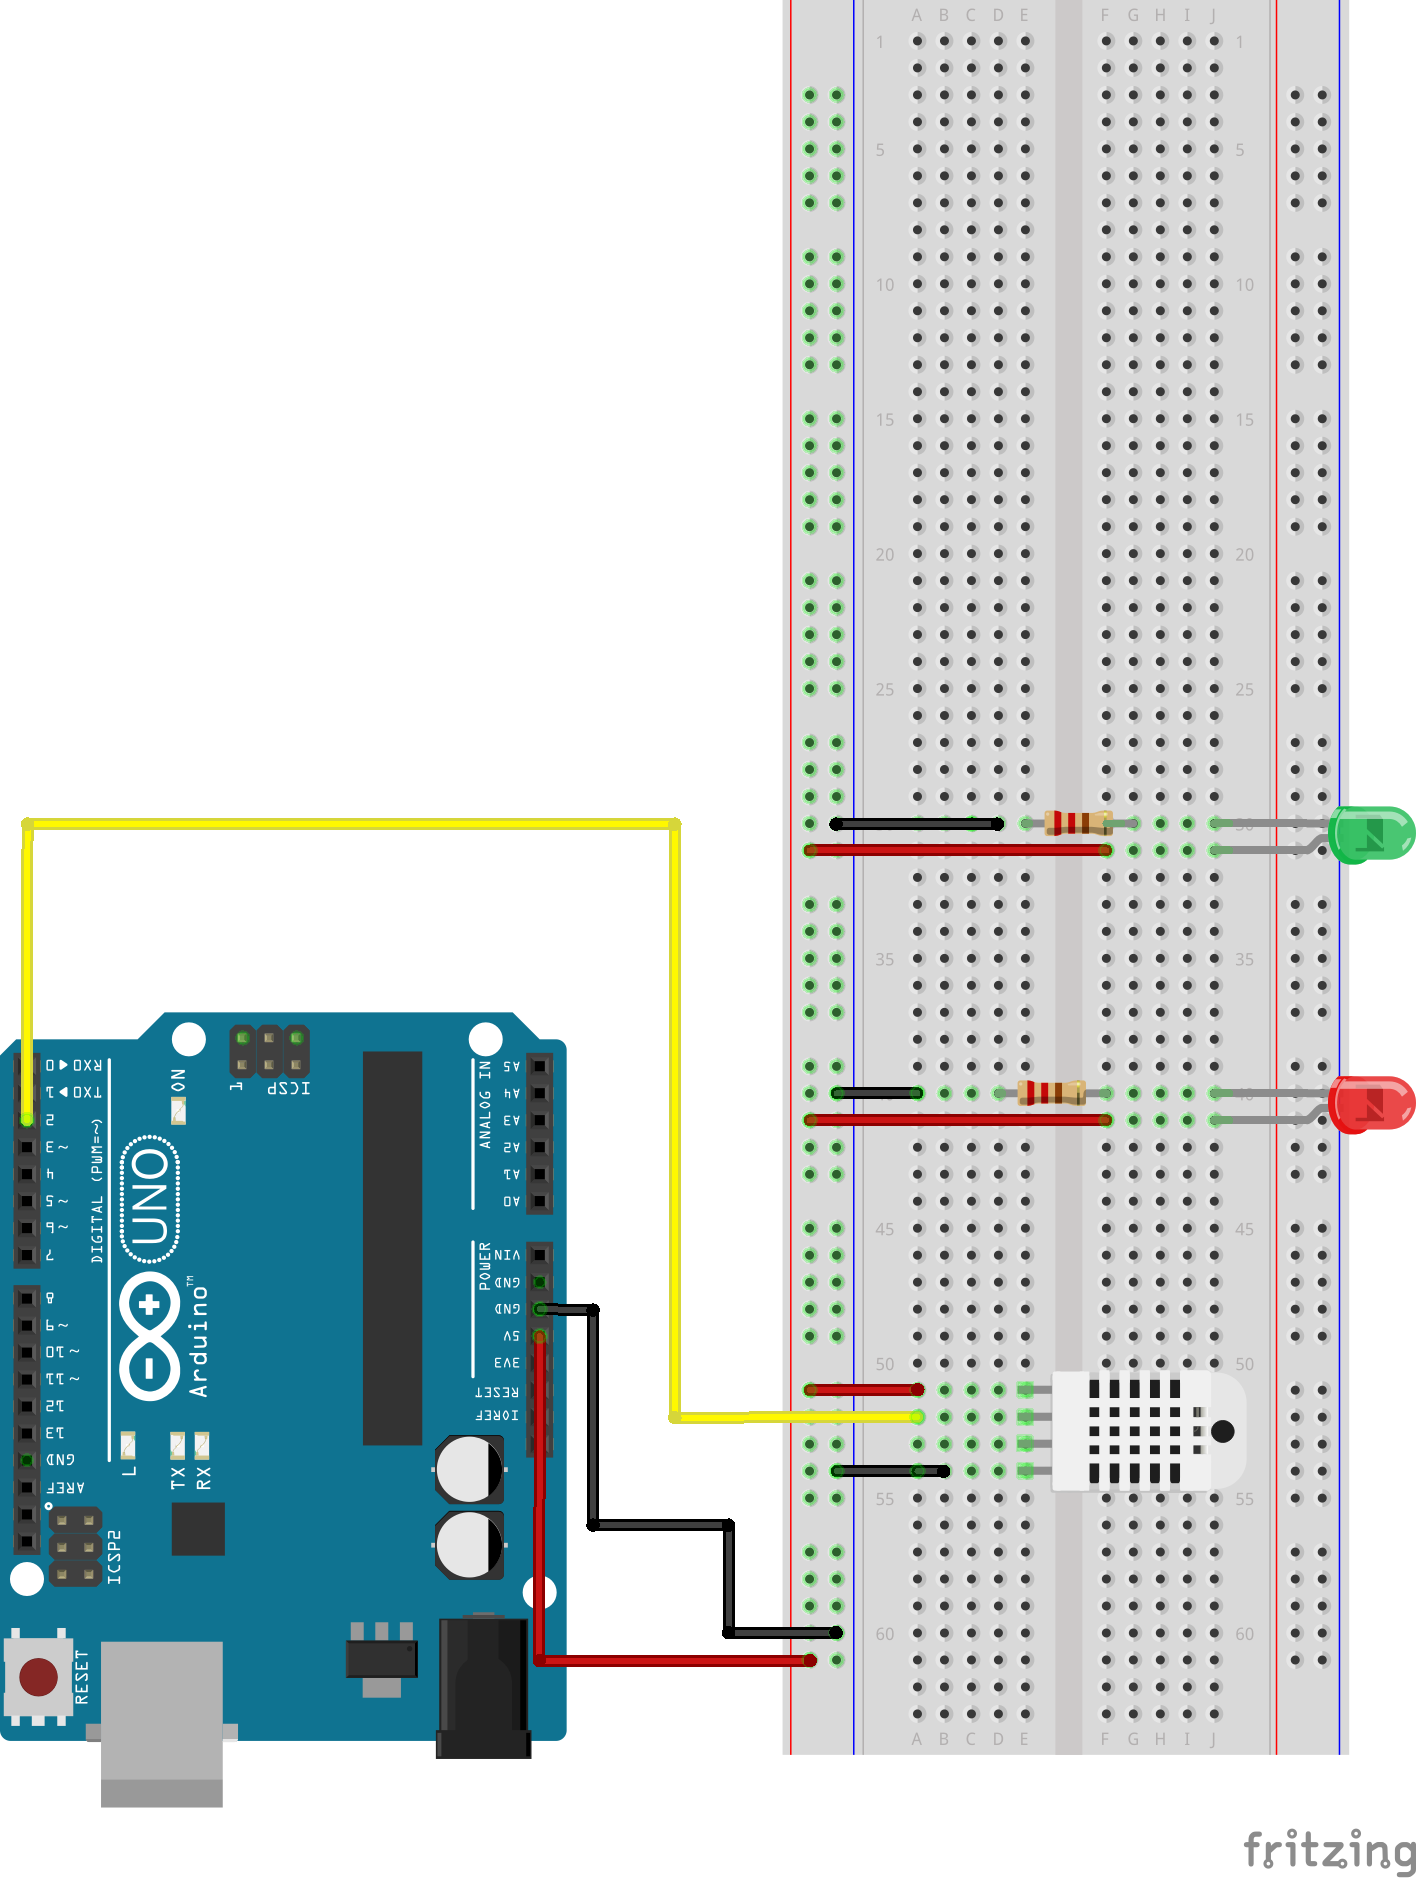
\includegraphics[width=0.5\textwidth]{pics/dhtled.png}
\caption{DHT und LEDs verbunden an Breadboard mit Arduino}
\end{center}
\end{figure}

\begin{python}
# @author Ugur Turhal

# This python file reads the serial port of the Arduino and
# reads the state of the LEDs out and Shows the Temperature

import numpy as np
import pandas as pd
import matplotlib.pyplot as plt
import serial
import time
import csv
from drawnow import *

plt.style.use('seaborn')
ser = serial.Serial('/dev/ttyACM0')
ser.flushInput()

ledRedPin = []
ledGreen = []
temperature = []


def makeFig():
    plt.close("all")
    plt.title('HIGH and LOW of \n selected pins')
    plt.ylim(0, 1.5, 0.4)
    plt.plot(ledRedPin, label='digitalRead_Red', color='red')
    plt.legend(bbox_to_anchor=(1.0, 0.5), loc='upper left')

    plt2 = plt.twinx()
    plt.ylim(0, 30, 6)
    plt2.plot(temperature, label='C')
    plt2.legend(bbox_to_anchor=(1.0, 1.01), loc='upper left')

    plt3 = plt.twinx();
    plt.ylim(0, 1.5)
    plt3.plot(ledGreen, label='digitalRead_Green', color='green')
    plt3.legend(bbox_to_anchor=(1.0, 0), loc='upper left')

    plt.tight_layout()
    plt.savefig("digitalRead.png")


def main():
    while True:
        ser_bytes = ser.readline()
        while ser.inWaiting() == 0:
            pass
        try:
            r = float(ser_bytes[0:1].decode("utf-8"));
            g = float(ser_bytes[1:len(ser_bytes) - 7].decode("utf-8"));
            temp = float(ser_bytes[3:len(ser_bytes)].decode("utf-8"));
            ledRedPin.append(r)
            temperature.append(temp)
            ledGreen.append(g)
            drawnow(makeFig)
        except:
            continue
            print("ERROR")
        with open("states.csv", "a") as f:
            writer = csv.writer(f, delimiter=",")
            writer.writerow([r, g, temp])


if __name__ == '__main__':
    print(main())

\end{python}
\begin{figure}[H]
\begin{center}
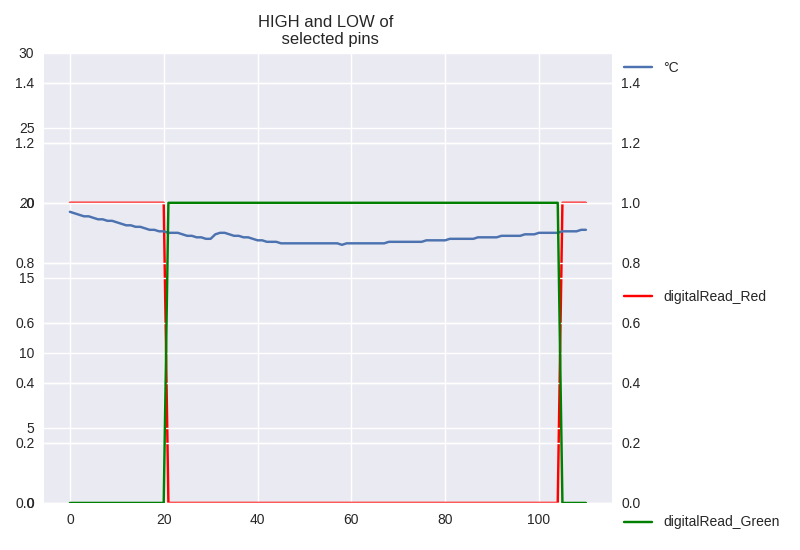
\includegraphics[width=0.7\textwidth]{pics/digitalRead.png}
\caption{HIGH und LOW bei bestimmten Temperaturen beim Auslesen des Serial Ports}
\end{center}
\end{figure}
Für die Erklärung der Abbildung 7 siehe: \url{https://github.com/ugurtu/CatcProject/blob/main/Bericht/bericht.pdf}
\end{document}
